	
\part{Cinética de crescimento}
	\chapter{SAXS resolvido no tempo}
	% todo: colocar os objetivos aqui, falar sobre correlações com ITC
	
	\section{Estudos preliminares}
	Antes de iniciar as medidas de SAXS resolvido no tempo, foram testadas várias amostras para observar qual é a combinação de surfactante e cossoluto com mais contraste, e que possui maior diferença entre os estados iniciais e finais. Foram escolhidos \CTAB, \TTAB{} e \DTAB{} com surfactantes, inicialmente, mas \CTAB{} foi descartado rapidamente pois a temperatura ambiente era menor do que o ponto Krafft do surfactante, e haveria a precipitação do mesmo dentro das seringas de injeção. Como cossoluto, escolheu-se NaSal, 4-clorobenzoato e 3,4-diclorobenzoato. Os cossolutos clorados apresentariam maior contraste, por possuírem maior densidade eletrônica, e por isso foram escolhidos.
	
	Foram preparadas soluções nas concentrações de 100 \mM{} de surfactante, que caracteriza o estado antes do crescimento, e 100 \mM{} de surfactante com 100 \mM{} do cossoluto, que caracteriza o estado depois do crescimento. Após o preparo e estabilização das amostras, as mesmas foram injetadas no capilar de \emph{flow-through} do equipamento. As curvas adquiridas estão na figura \ref{fig:ft_preliminar}. Não foi incluído a mistura 3,4-diclorobenzoato e surfactante, pois o contraste era muito baixo, e não havia uma boa relação sinal-ruído.
	
	\begin{figure}[h]
		\centering
		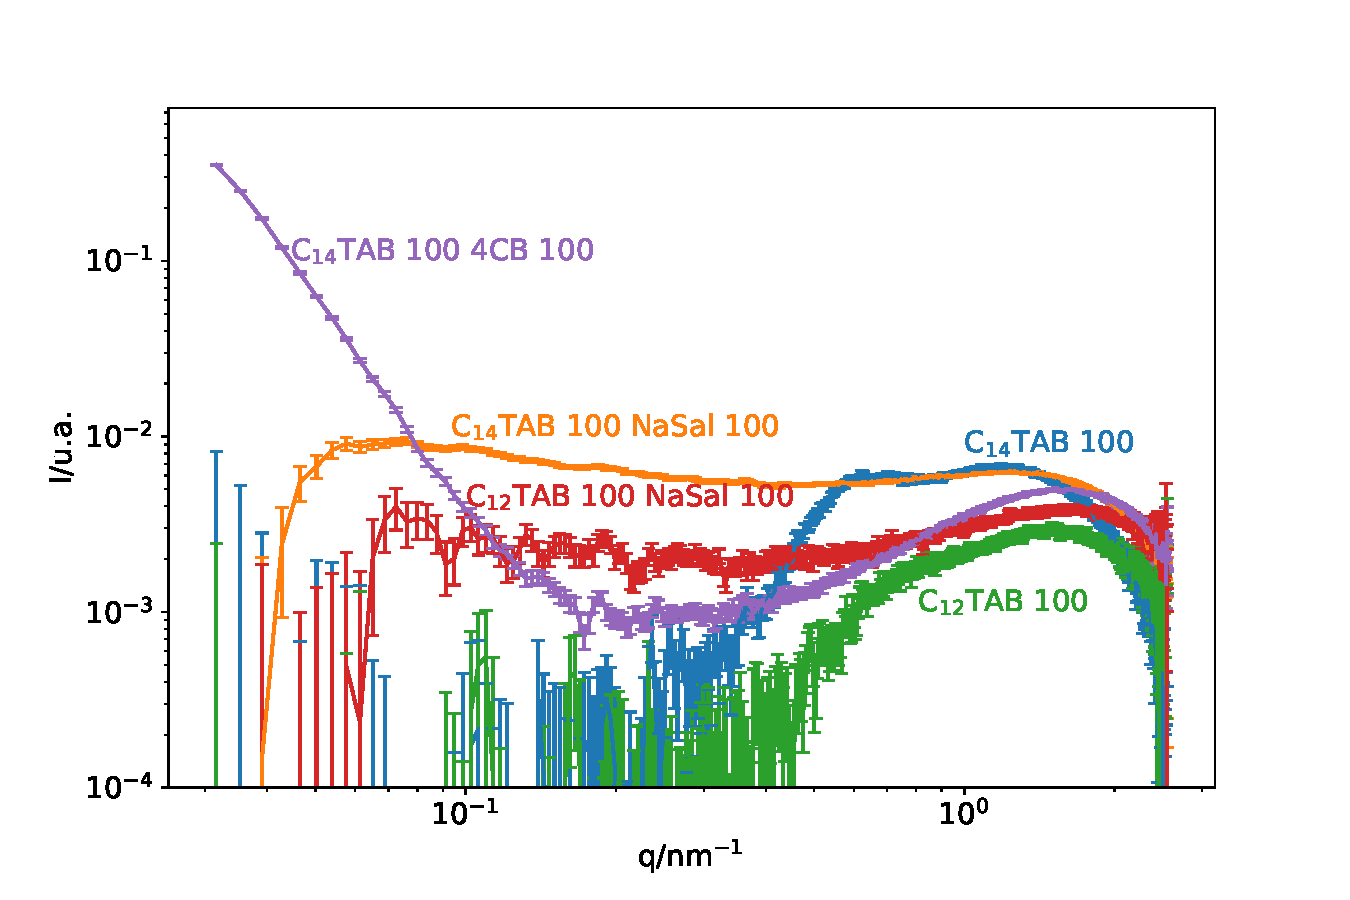
\includegraphics[width=0.7\textwidth]{imagens/saxs/FT_amostras}
		\caption{Curvas de SAXS para várias misturas de surfactantes e cossolutos, com 100 ms de tempo de integração.}
		\label{fig:ft_preliminar}
	\end{figure}

	Observando as curvas, é possível notar que a diferença entre os estados iniciais e finais de \DTAB{} não são muito diferentes, possivelmente porque as micelas formadas não possuem um comprimento muito significativo. Já a diferença entre os estados iniciais e finais para \TTAB{} é bastante pronunciada. Um gráfico comparativo foi criado, realçando as regiões de maior importância (\ref{fig:tr_comparacao_ttab}).
	
	\begin{figure}[h]
		\centering
		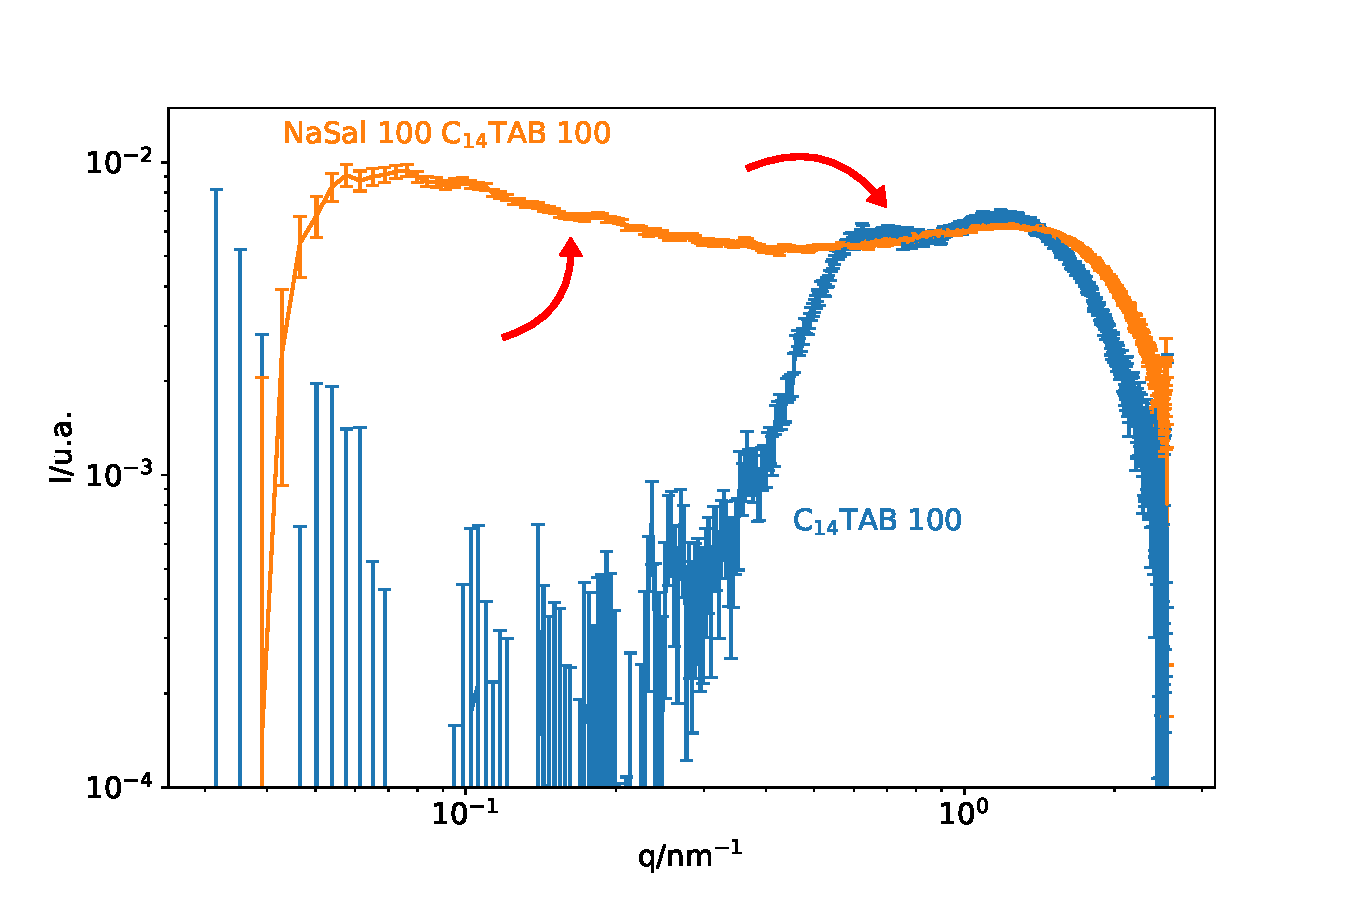
\includegraphics[width=0.7\textwidth]{imagens/saxs/tr_comparacao_antes_depois}
		\caption{Curvas de SAXS para amostras de TTAB 100\mM{} (antes) e 100 \mM de TTAB com 100 \mM{} de NaSal (depois). As setas indicam as regiões onde será observada a maior diferença nas curvas.}
		\label{fig:tr_comparacao_ttab}
	\end{figure}
	
	A região em baixos valores de \q{} é bastante ruidosa na amostra com TTAB 100 \mM{} devido ao baixo contraste entre a amostra e o \emph{background}. O mesmo ocorre na amostra com micelas gigantes de NaSal e TTAB, e a queda na curva não possui significado físico. Isso será importante na discussão, pois observar-se-á que essa região terá um decaimento em \(q^{-4}\), que pode não ter significado físico, e é um artefato oriundo do baixo contraste. É interessante notar a semelhança entre o perfil de espalhamento obtido aqui e na figura \ref{fig:SAXS_micelas_esfericas}, obtido na linha SAXS1 do LNLS. A principal diferença é uma faixa de \q{} menor, que fornece informações sobre estruturas maiores, o que é mais apropriado ao estudo de micelas gigantes.
	
	\section{TR-SAXS}
	
	Com essas informações, foram medidas várias misturas de TTAB e NaSal, nas proporções de 55:55, 75:75, 100:100 e 60:100 de NaSal:TTAB. Todas as concentrações estão em \mM. Com essas variações de concentração, era esperado observar mudanças na cinética de crescimento. A amostra com 60:100 NaSal:TTAB foi escolhida por possuir uma carga positiva e, consequentemente, resultar numa solução micelar mais viscosa, cujo crescimento poderia ser mais lento também. Essa última amostra foi medida em duas distâncias de detector, 3 m e 1,5 m, para ver se isso afetava os resultados dos ajustes. Todas as outras amostras foram medidas com o detector a 3 m de distância.
	
	Várias combinações de tempos de espera foram estudadas, e no final concluiu-se que os parâmetros disponíveis na tabela \ref{tab:ccdmvdc_par} forneceram a melhor razão sinal-ruído com o menor tempo possível de integração. Com esses parâmetros pode-se calcular o tempo desde a mistura inicial até um determinado \emph{frame}. Para as amostras analisadas, os tempos do início de cada \emph{frame} estão na tabela \ref{tab:tr_tempos_frames}.
	
				\begin{table}[h]
		\IBGEtab{%
			\caption{Tempos de mistura no início de cada \emph{frame} para as análises de SAXS resolvido no tempo}
			\label{tab:tr_tempos_frames}
		}%
		{%
			\begin{tabular}{c c | c c | c c | c c | c c}
				\toprule
				Frame & Tempo/s & Frame & Tempo/s & Frame & Tempo/s & Frame & Tempo/s & Frame & Tempo/s \\ \midrule
				  1   & 0.035   & 7     & 0.249   & 13    & 0.583   & 19    & 1.127   & 25    & 2.045   \\
				  2   & 0.065   & 8     & 0.295   & 14    & 0.655   & 20    & 1.248   & 26    & 2.252   \\
				  3   & 0.097   & 9     & 0.344   & 15    & 0.734   & 21    & 1.380   & 27    & 2.479   \\
				  4   & 0.131   & 10    & 0.397   & 16    & 0.820   & 22    & 1.525   & 28    & 2.727   \\
				  5   & 0.168   & 11    & 0.454   & 17    & 0.914   & 23    & 1.683   & 29    & 2.999   \\
				  6   & 0.207   & 12    & 0.516   & 18    & 1.016   & 24    & 1.856   & 30    & 3.298	\\ \bottomrule
			\end{tabular}
		}{}
	\end{table}  
	
	Cada combinação NaSal:TTAB foi analisada no mínimo 5 vezes, e foi feita uma média das curvas, com propagação de erro. Cada curva foi analisada pelo software SUPERSAXS. As figuras \ref{fig:saxs_tr_55} -- \ref{fig:saxs_tr_60_15} mostram os dados obtidos e os ajustes de cada uma das curvas médias. As curvas estão coloridas de modo que as primeiras estejam em tons escuros e as últimas, em tons claros. Os números dos \emph{frames} estão juntos de cada cor em cada figura.
	
	\begin{figure}[h]
		\begin{subfigure}[t]{0.5\textwidth}
			\centering
			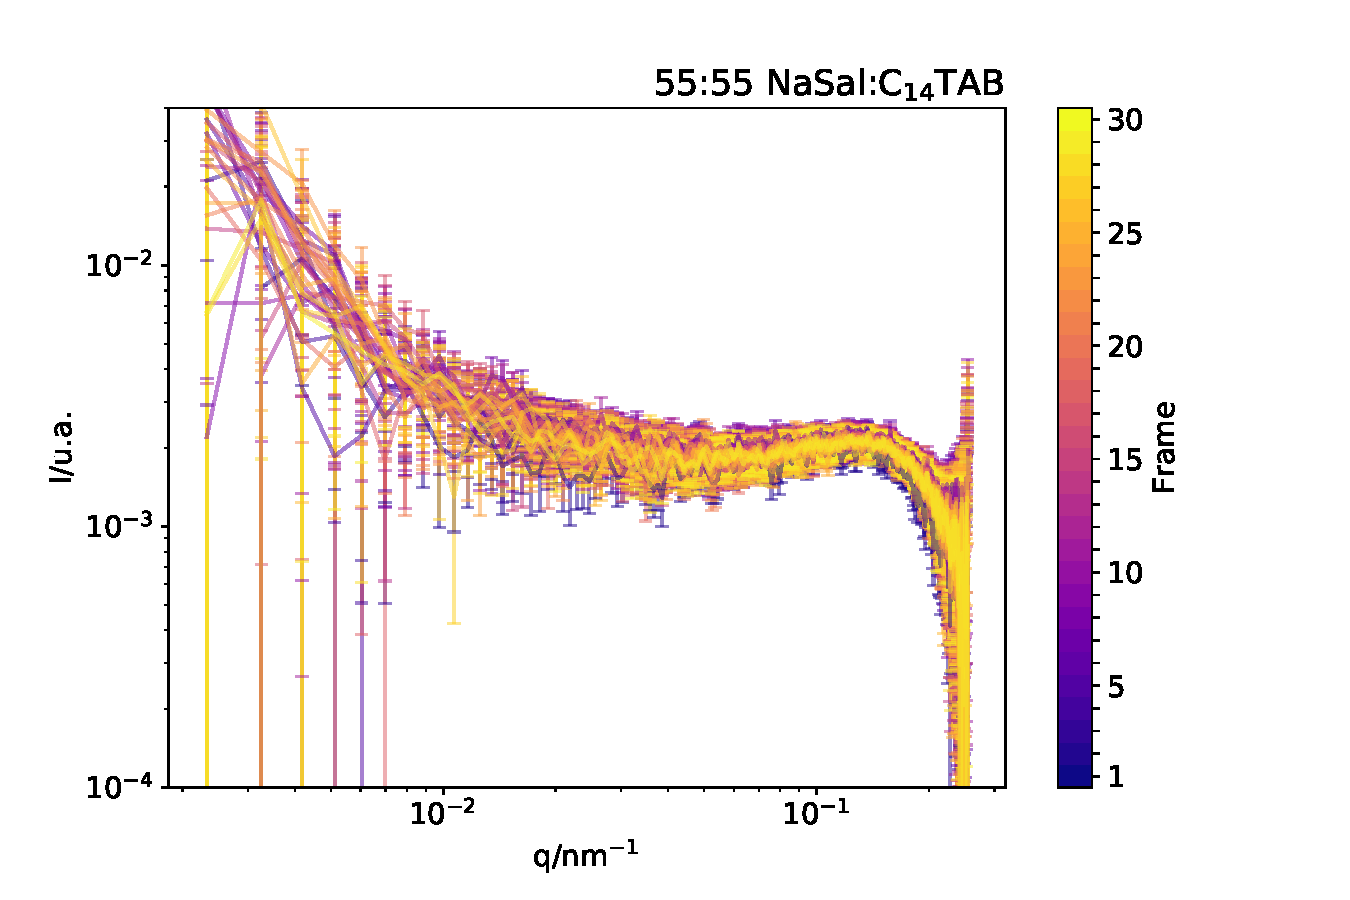
\includegraphics[width=\textwidth]{imagens/saxs/TR_saxs_55_55_dados.pdf}
			\caption{Dados}
			\label{fig:saxs_tr_55_d}
		\end{subfigure}%
		\begin{subfigure}[t]{0.5\textwidth}
			\centering
			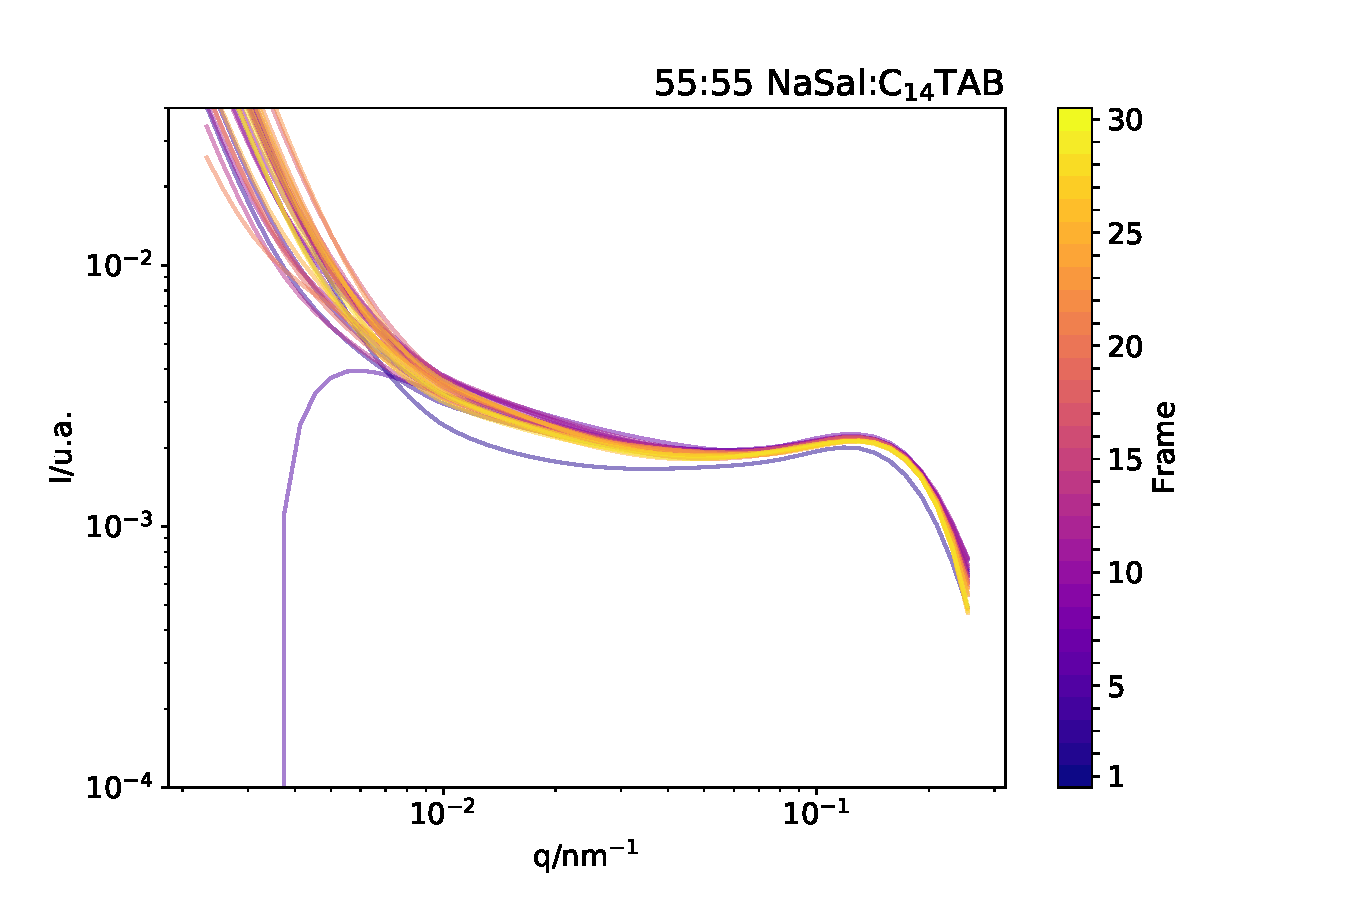
\includegraphics[width=\textwidth]{imagens/saxs/TR_saxs_55_55_ajuste.pdf}
			\caption{Ajustes}
			\label{fig:saxs_tr_55_a}
		\end{subfigure}
		\caption{Dados experimentais médios das curvas de SAXS nas aquisições numeradas de 1-30, numeradas do menor ao maior tempo de espera. As curvas foram obtidas pela mistura de 55 \mM{} de NaSal com 55\mM{} de TTAB.}
		\label{fig:saxs_tr_55}
	\end{figure} 

	\begin{figure}[h]
		\begin{subfigure}[t]{0.5\textwidth}
			\centering
			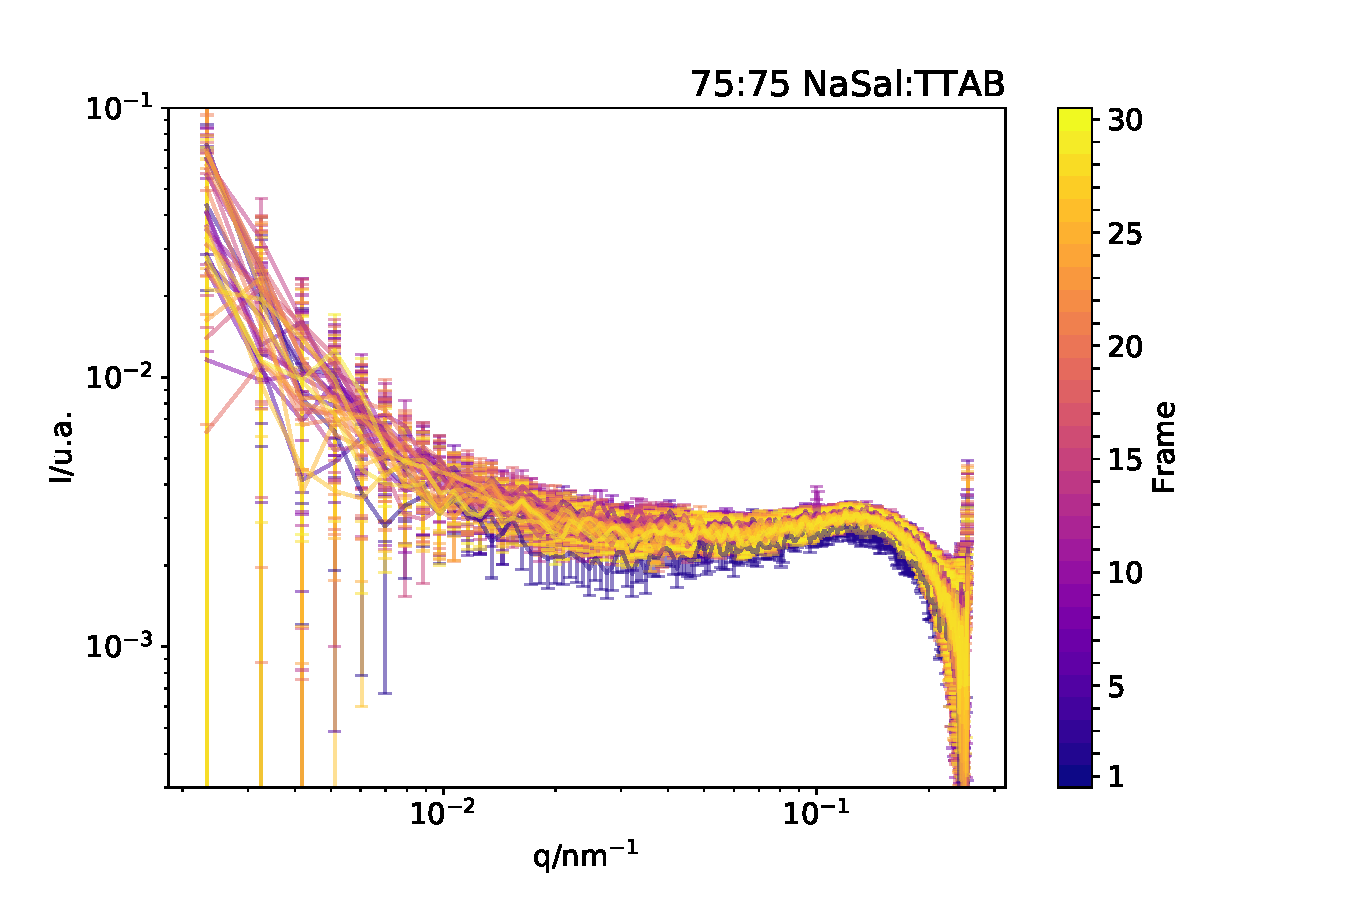
\includegraphics[width=\textwidth]{imagens/saxs/TR_saxs_75_75_dados.pdf}
			\caption{Dados}
			\label{fig:saxs_tr_75_d}
		\end{subfigure}%
		\begin{subfigure}[t]{0.5\textwidth}
			\centering
			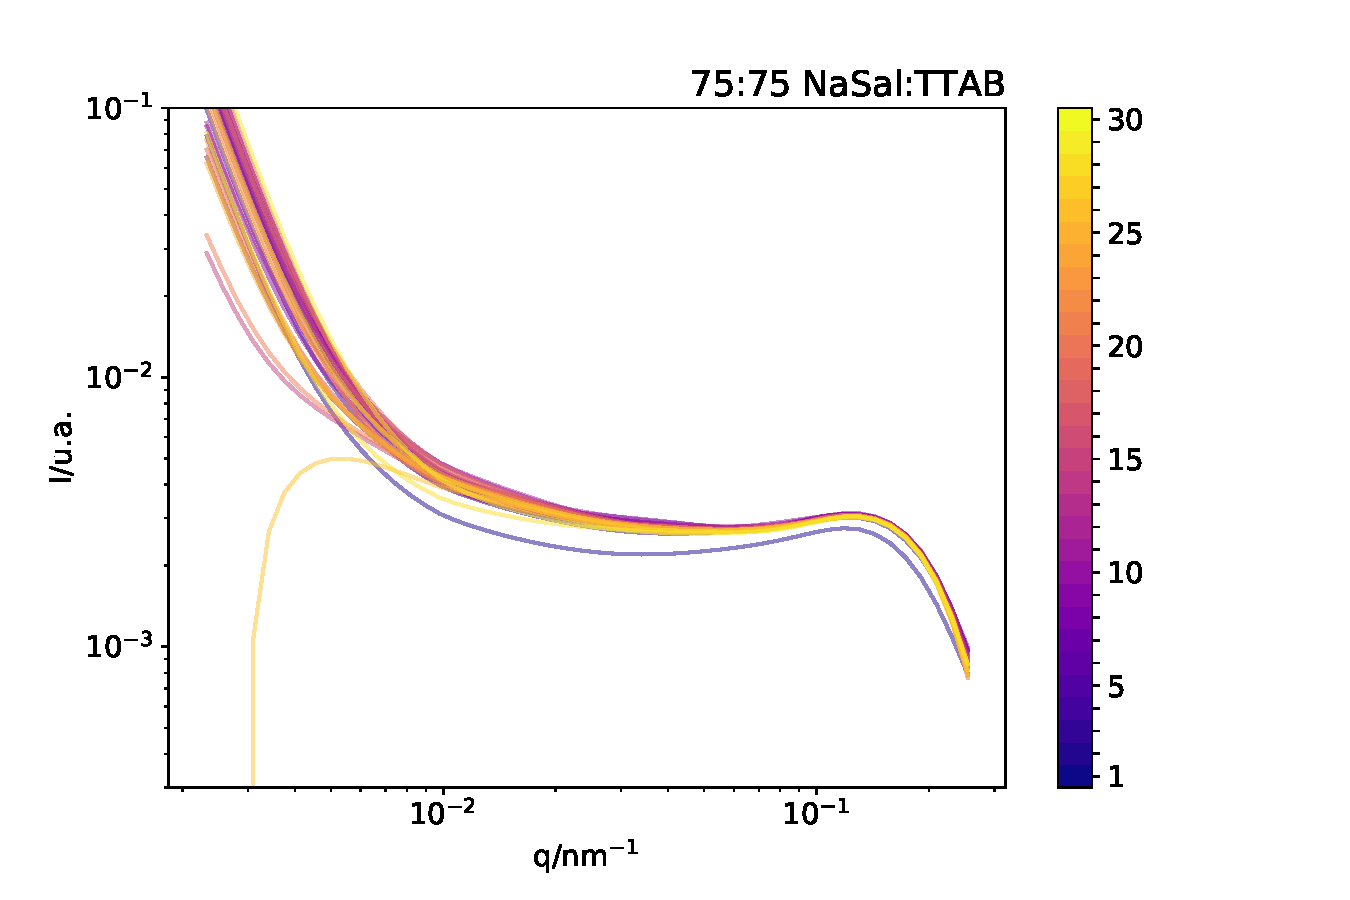
\includegraphics[width=\textwidth]{imagens/saxs/TR_saxs_75_75_ajuste.pdf}
			\caption{Ajustes}
			\label{fig:saxs_tr_a}
		\end{subfigure}
		\caption{Dados experimentais médios das curvas de SAXS nas aquisições numeradas de 1-30, numeradas do menor ao maior tempo de espera. As curvas foram obtidas pela mistura de 75 \mM{} de NaSal com 75 \mM{} de TTAB.}
		\label{fig:saxs_tr_75}
	\end{figure} 
	
	\begin{figure}[h]
		\begin{subfigure}[t]{0.5\textwidth}
			\centering
			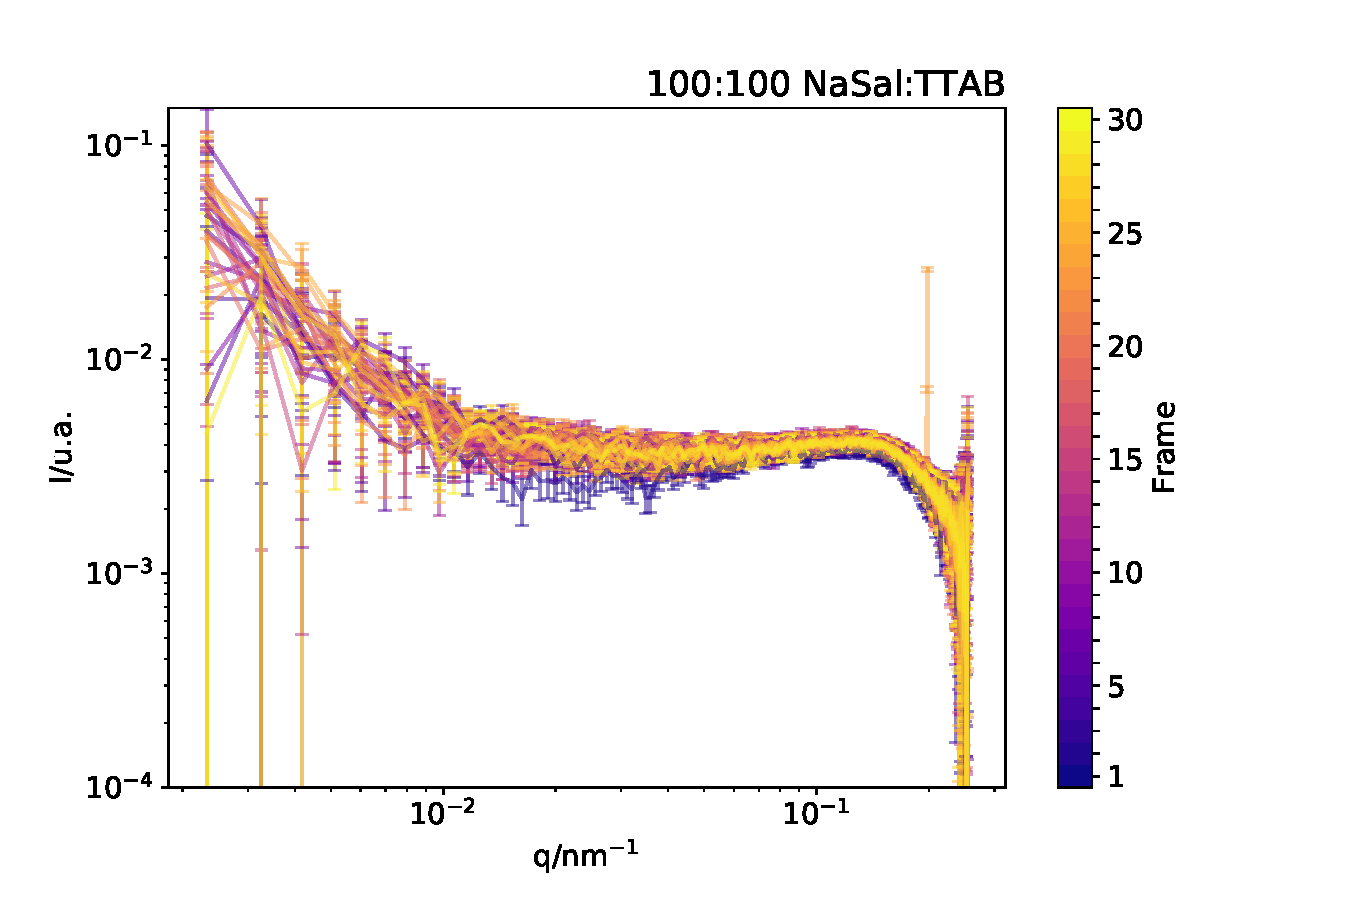
\includegraphics[width=\textwidth]{imagens/saxs/TR_saxs_100_100_dados.pdf}
			\caption{Dados}
			\label{fig:saxs_tr_100_d}
		\end{subfigure}%
		\begin{subfigure}[t]{0.5\textwidth}
			\centering
			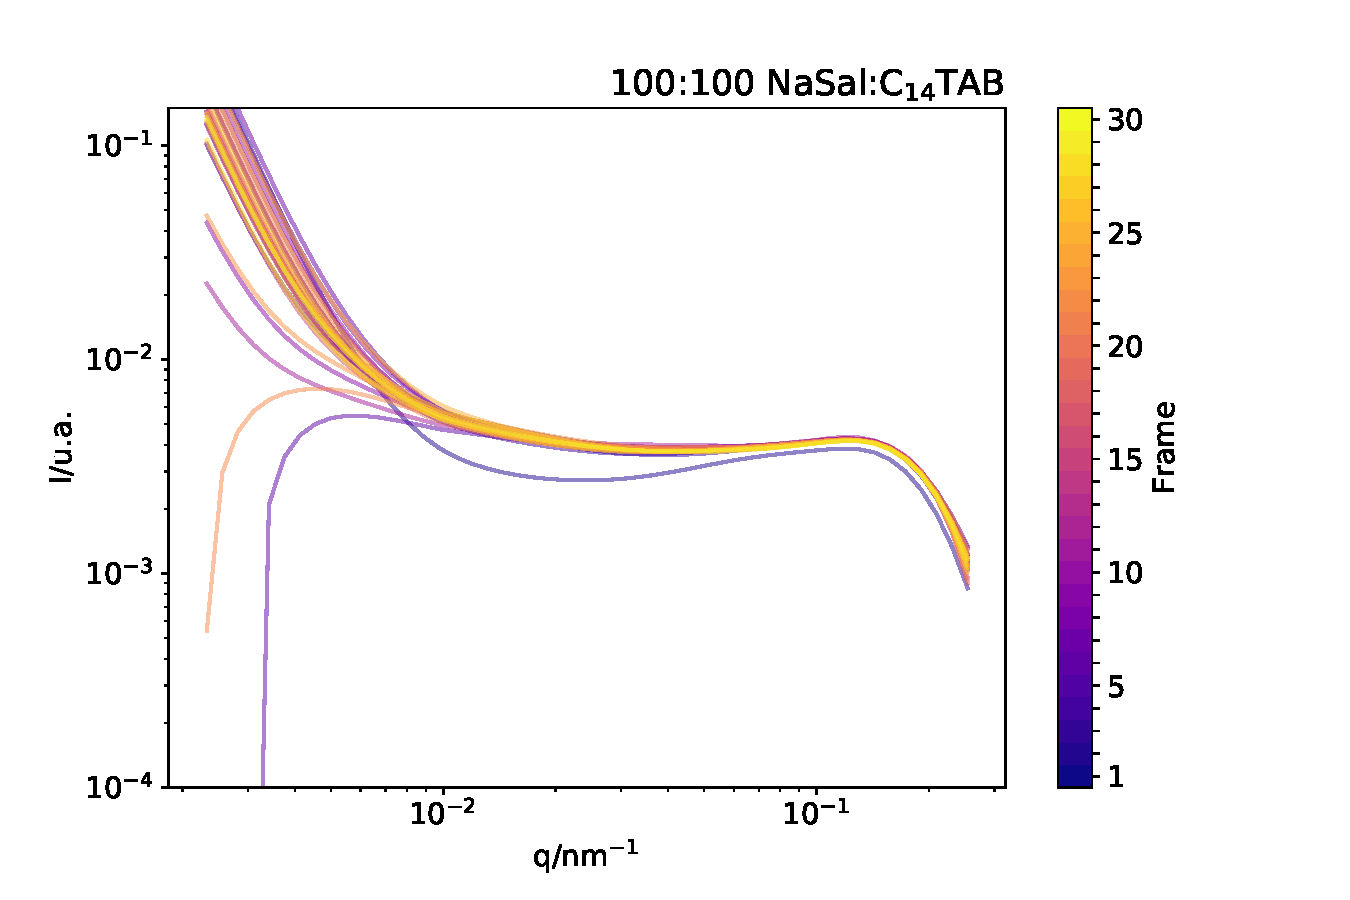
\includegraphics[width=\textwidth]{imagens/saxs/TR_saxs_100_100_ajustes.pdf}
			\caption{Ajustes}
			\label{fig:saxs_tr_100_a}
		\end{subfigure}
		\caption{Dados experimentais médios das curvas de SAXS nas aquisições numeradas de 1-30, numeradas do menor ao maior tempo de espera. As curvas foram obtidas pela mistura de 100 \mM{} de NaSal com 100 \mM{} de TTAB.}
		\label{fig:saxs_tr_100}
	\end{figure} 
	
	\begin{figure}[h]
		\begin{subfigure}[t]{0.5\textwidth}
			\centering
			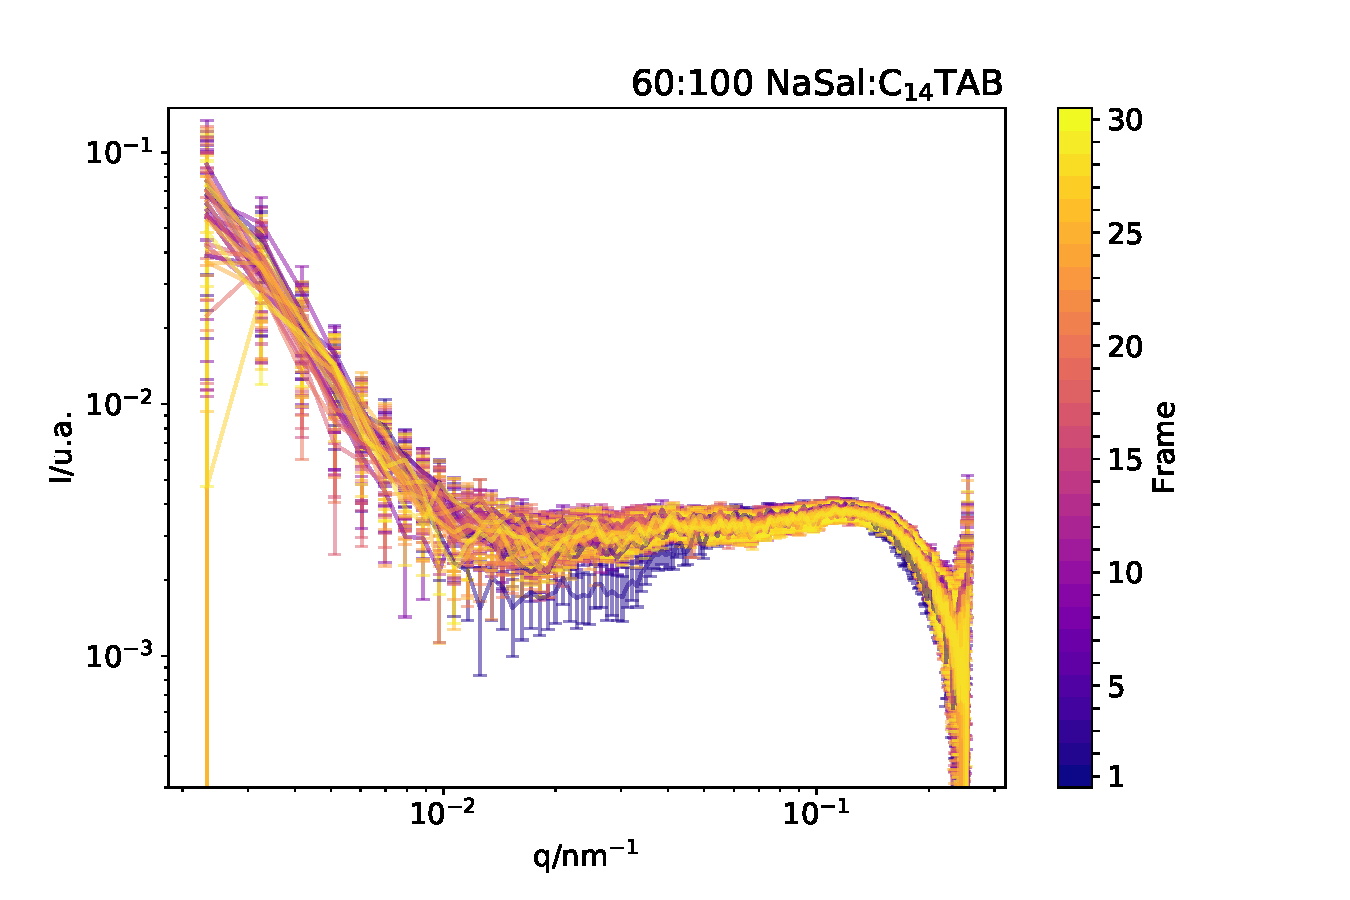
\includegraphics[width=\textwidth]{imagens/saxs/TR_saxs_60_100_3_dados.pdf}
			\caption{Dados}
			\label{fig:saxs_tr_60_3_d}
		\end{subfigure}%
		\begin{subfigure}[t]{0.5\textwidth}
			\centering
			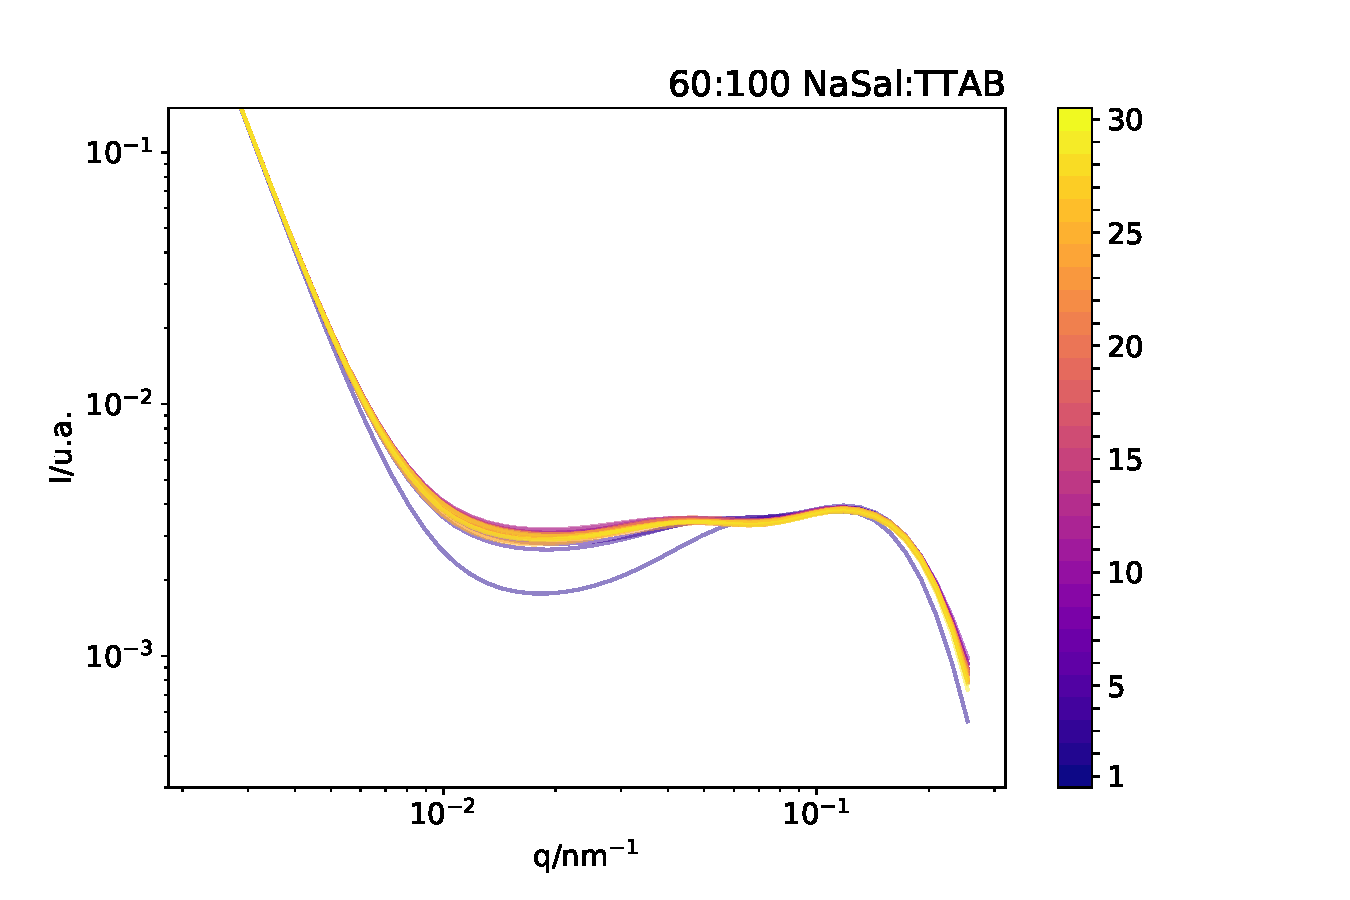
\includegraphics[width=\textwidth]{imagens/saxs/TR_saxs_60_100_3_ajustes.pdf}
			\caption{Ajustes}
			\label{fig:saxs_tr_60_3_a}
		\end{subfigure}
		\caption{Dados experimentais médios das curvas de SAXS nas aquisições numeradas de 1-30, numeradas do menor ao maior tempo de espera. As curvas foram obtidas pela mistura de 60 \mM{} de NaSal com 100 \mM{} de TTAB.}
		\label{fig:saxs_tr_60_3}
	\end{figure} 

	\begin{figure}[h]
		\begin{subfigure}[t]{0.5\textwidth}
			\centering
			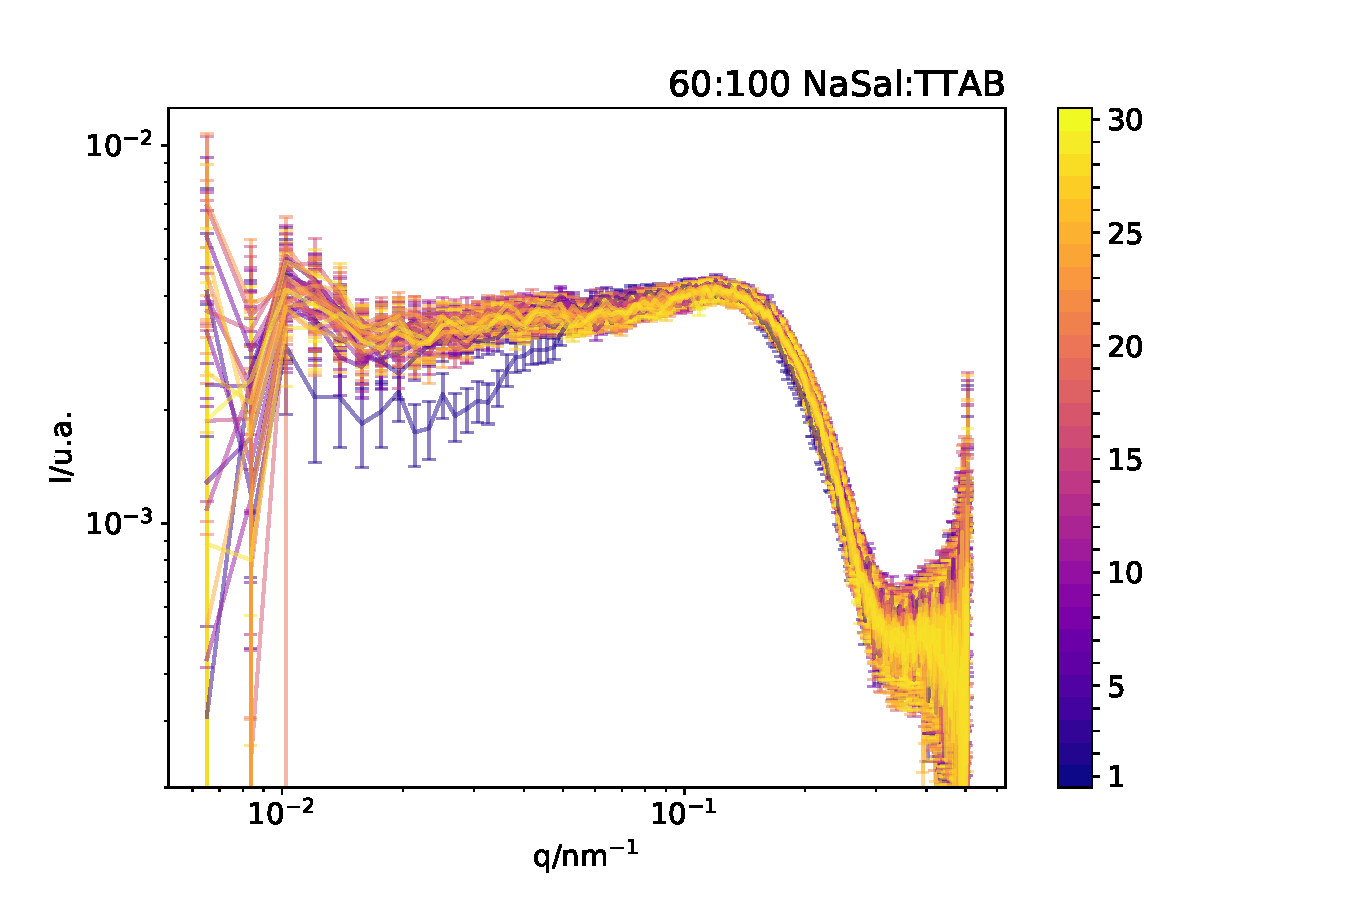
\includegraphics[width=\textwidth]{imagens/saxs/TR_saxs_60_100_15_dados.pdf}
			\caption{Dados}
			\label{fig:saxs_tr_60_15_d}
		\end{subfigure}%
		\begin{subfigure}[t]{0.5\textwidth}
			\centering
			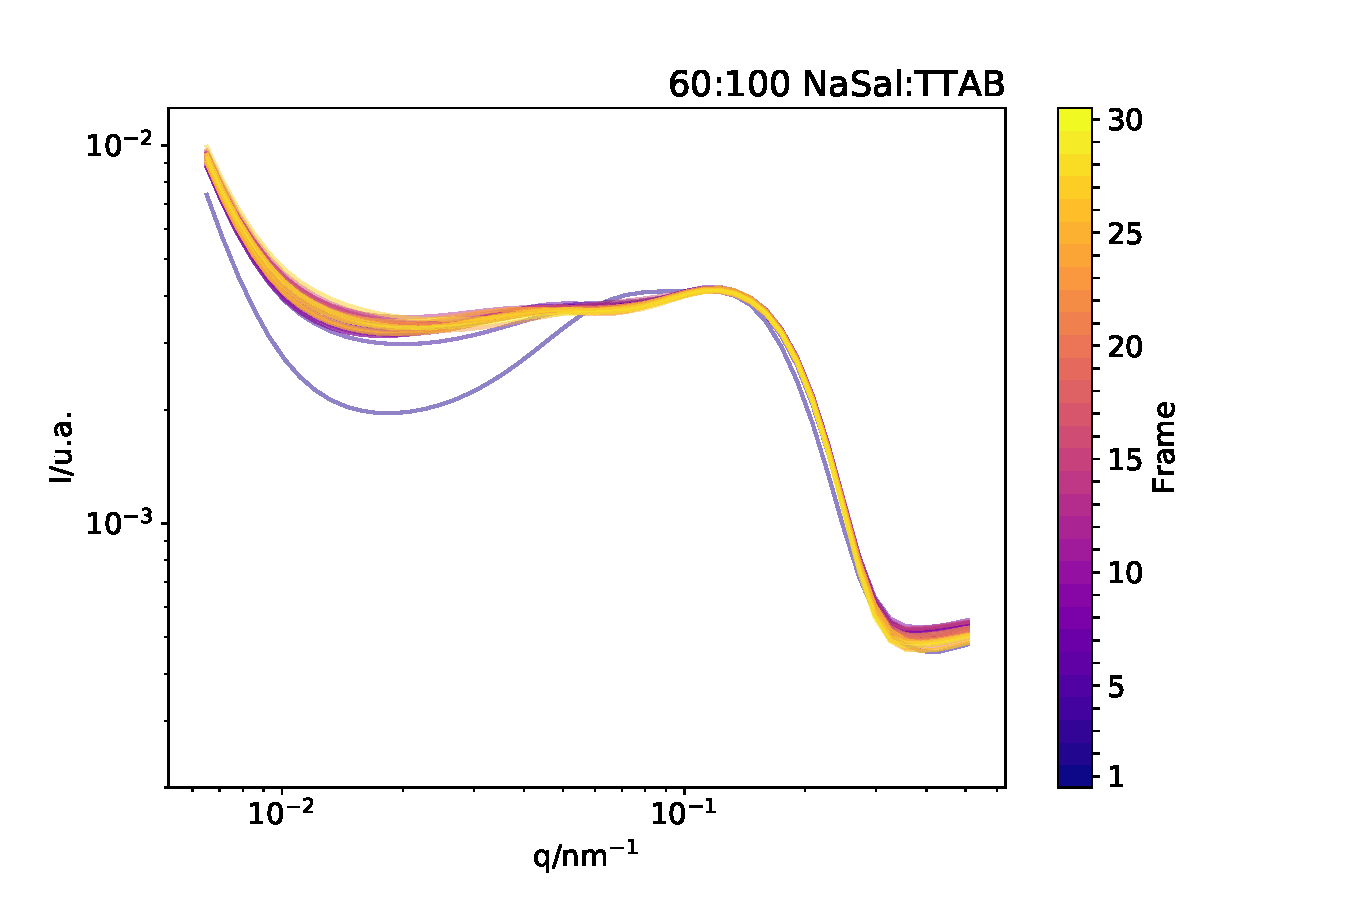
\includegraphics[width=\textwidth]{imagens/saxs/TR_saxs_60_100_15_ajustes.pdf}
			\caption{Ajustes}
			\label{fig:saxs_tr_60_15_a}
		\end{subfigure}
		\caption{Dados experimentais médios das curvas de SAXS nas aquisições numeradas de 1-30, numeradas do menor ao maior tempo de espera. As curvas foram obtidas pela mistura de 60 \mM{} de NaSal com 60 \mM{} de TTAB. Neste caso, a distância do detector é de 1,5m, abrangendo uma faixa de \q{} diferente.}
		\label{fig:saxs_tr_60_15}
	\end{figure} 
	
%	\FloatBarrier
	
	Todos os primeiros \emph{frames} das curvas possuem um formato diferente dos demais, que é mais pronunciado à medida que a concentração aumenta. Isso mostra que em 35 ms, as micelas possuíam uma estrutura diferente do que em 65 ms, e adiante. Essas curvas são, todavia, bastante próximas em formato ao estado final da figura \ref{fig:tr_comparacao_ttab}, o que significa que o crescimento micelar está quase completo em 35 ms e se completa em 65 ms. Uma possível explicação para esse acontecimento é a alta concentração de micelas no meio. Isso acelera a cinética de colisão entre micelas e cossolutos. Além disso, a rede micelar pode se tornar tão densa que o meio se torna homogêneo para SAXS, e não é possível distinguir entre uma micela e outra.
	
	Na maior parte das curvas, é possível observar que na região de baixo \q, há um decaimento exponencial. O modelo utilizado não prevê esse comportamento, que teve de ser incluído externamente. O valor do expoente, em todos os ajustes, foi de 4, isso é, \( \^{-4} \). Se essa região for verdadeira, a validade do modelo utilizado para o tratamento se torna questionável. Porém, essa queda não foi observada na cela de \emph{flow-through}, como mencionado anteriormente. Além disso, houveram ligeiras variações no valor do \emph{background} entre cada amostra, devido à limpeza, apesar de que se garantiu que nenhum sinal significativo era observado. A figura \ref{fig:problema_limpeza} mostra a minúscula diferença entre o \emph{background}, medido com o capilar seco e vazio, e o capilar após a primeira limpeza com água. Essa pequena diferença pode gerar o sinal em baixo \q{} com o decaimento observado devido à baixa intensidade nos sinais, devido ao curto tempo de integração, necessário para medidas cinéticas, e o baixo contraste entre as micelas e o solvente. Logo, a região em baixo \q{}, provavelmente, não possui significado físico, e o decaimento exponencial utilizado é somente um artifício matemático para auxiliar no ajuste das curvas.
	
	\begin{figure}[h]
		\centering
		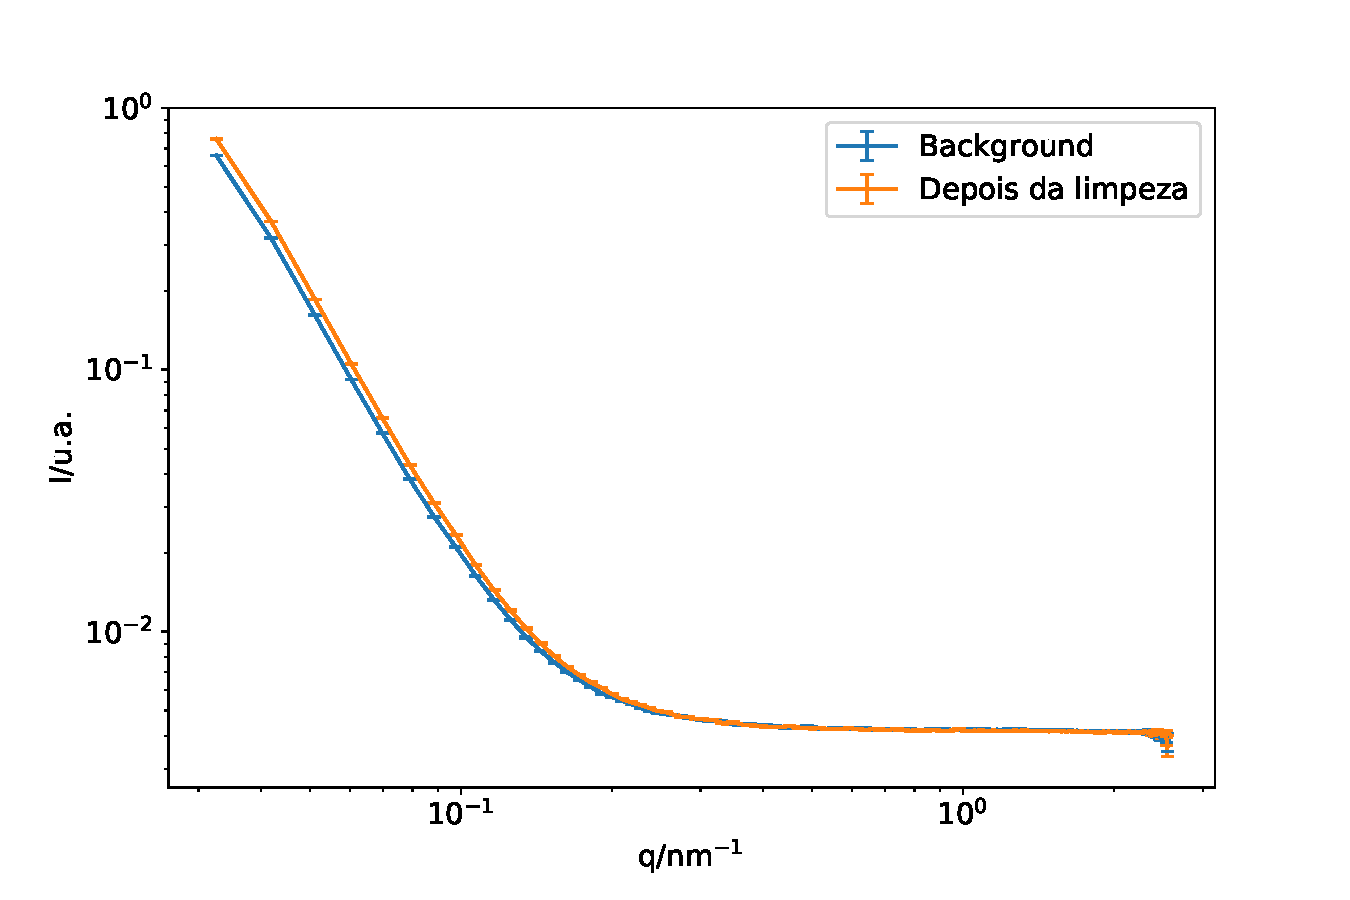
\includegraphics[width=0.7\textwidth]{imagens/saxs/problema_limpeza}
		\caption{Diferença entre o sinal de SAXS do \emph{background} e após a limpeza com água.}
		\label{fig:problema_limpeza}
	\end{figure}

	Os resultados dos ajustes se encontram nas figuras \ref{fig:params_dhead_radcore}, \ref{fig:params_nurpa_dcq} e \ref{fig:params_scale_rhorel}. A tabela \ref{tab:params_ajuste_saxs} resume as mesmas informações. Parte dos parâmetros de ajuste não foram variados, para auxiliar na convergência. Por exemplo, o comprimento de Kuhn e de contorno foram fixados em 1000 nm e 5000 nm, respectivamente, pois a alteração de qualquer um não resultava numa alteração significativa das curvas. Isso significa que não foi possível observar a cinética de mudança do comprimento das micelas por essa técnica. As diferenças nos formatos das curvas se devem a outros parâmetros.
		
		% TODO: esses parâmetros são em nm ou em angstrom? Checar no código pra ver se ele converte de nm pra A ou ao contrário. Qual é o raio de uma micela?
		
	\begin{figure}
		\begin{subfigure}[t]{0.5\textwidth}
			\centering
			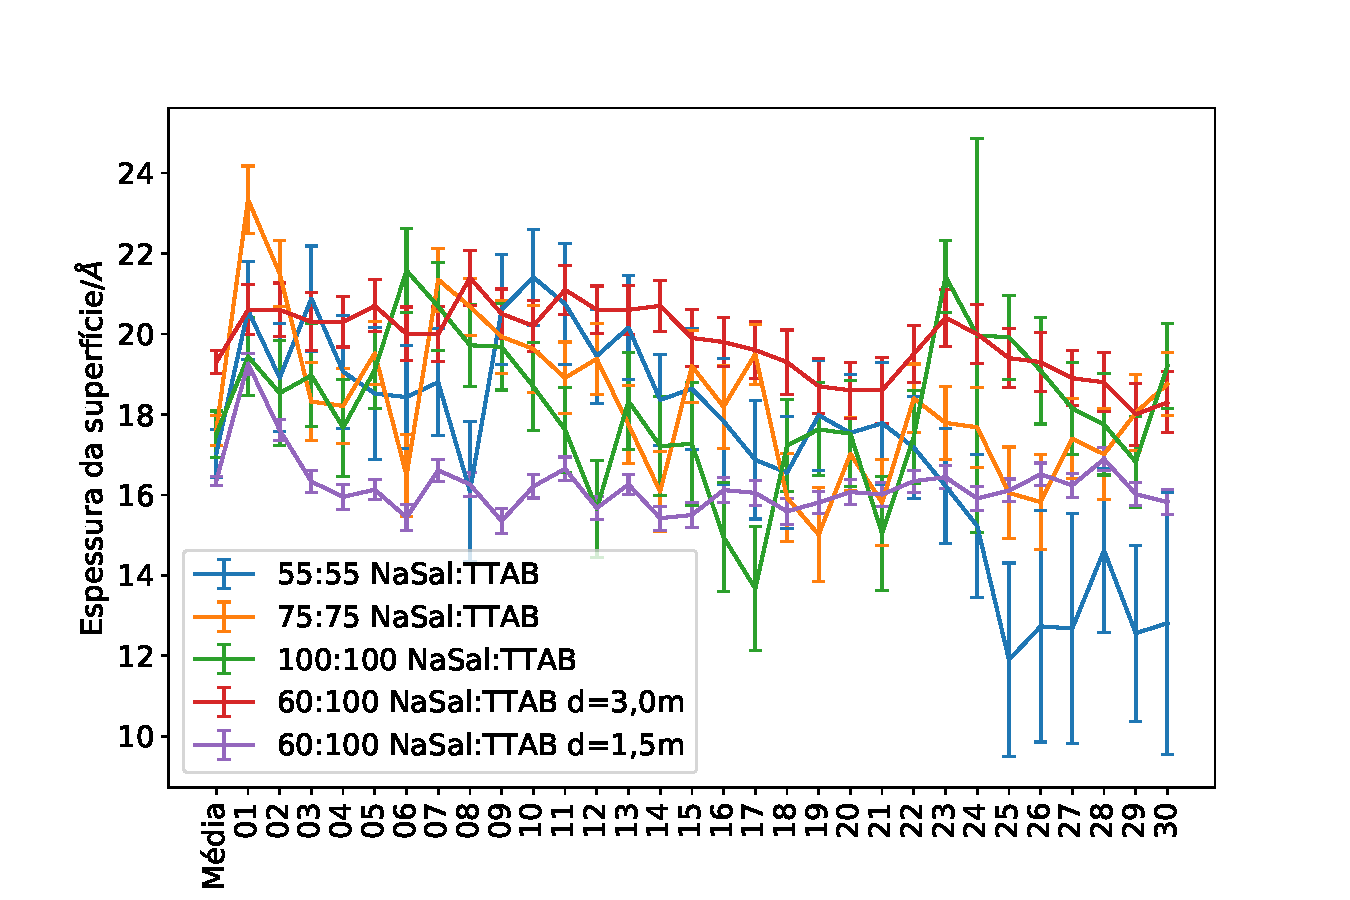
\includegraphics[width=\textwidth]{imagens/saxs/param_d_head}
			\caption{Espessura da superfície, \(d_{head}\)}
			\label{fig:param_dhead}
		\end{subfigure} %
		\begin{subfigure}[t]{0.5\textwidth}
			\centering
			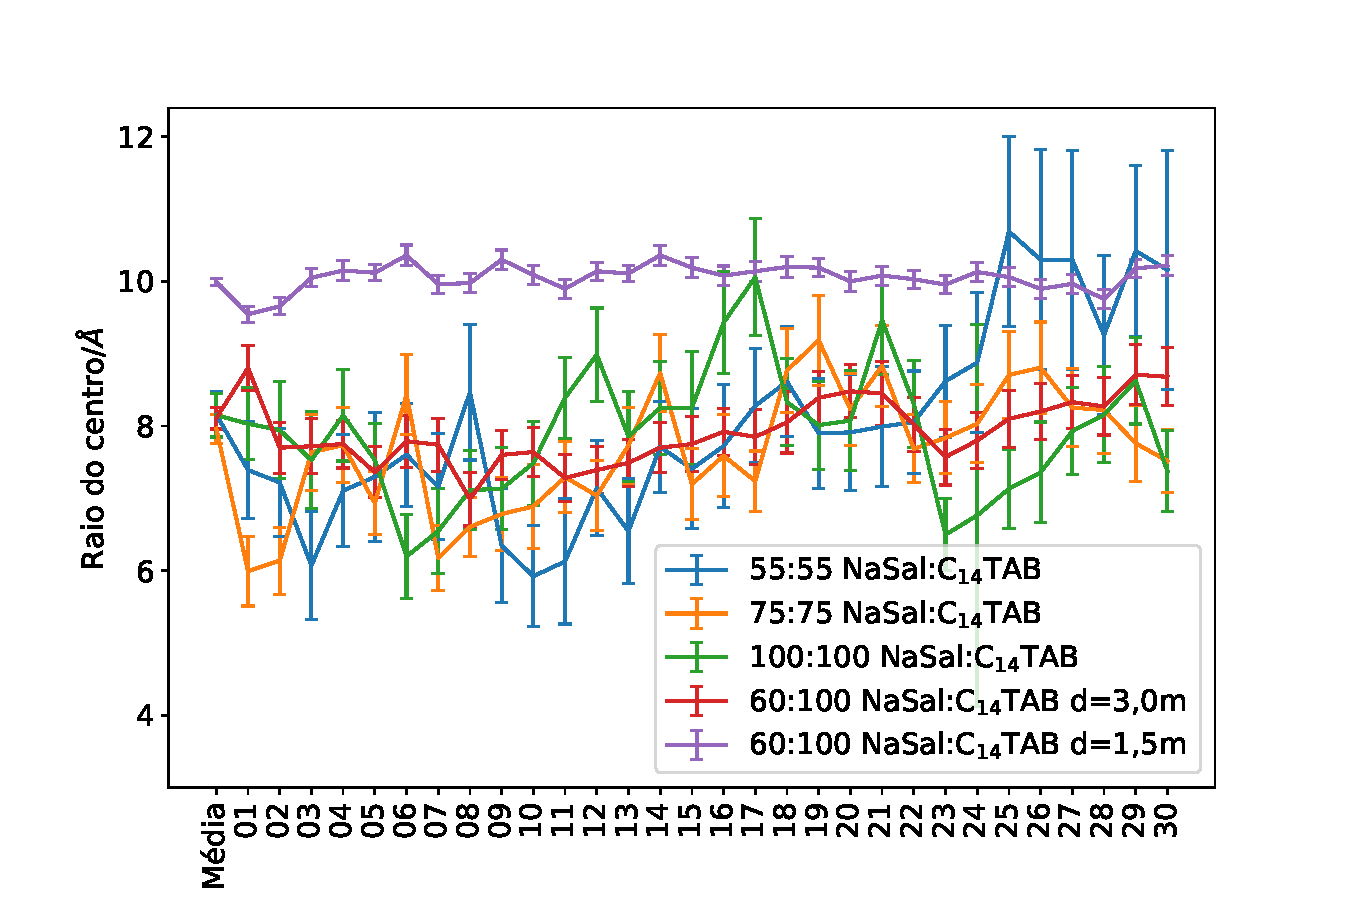
\includegraphics[width=\textwidth]{imagens/saxs/param_rad_core}
			\caption{Raio do \(\r_{core}\)}
			\label{fig:param_radcore}
		\end{subfigure}
		\caption{Parâmetros \(d_{head}\) e \(r_{core}\), ambos em nm, das cinco amostras medidas. Os números indicam o \emph{frame}, e o tempo após a mistura pode ser checada na tabela \ref{tab:tr_tempos_frames}. ``Média'' significa o resultado do ajuste da média das curvas 2-30, que eram praticamente idênticas.}
		\label{fig:params_dhead_radcore}
	\end{figure}

	\begin{figure}
		\begin{subfigure}[t]{0.5\textwidth}
			\centering
			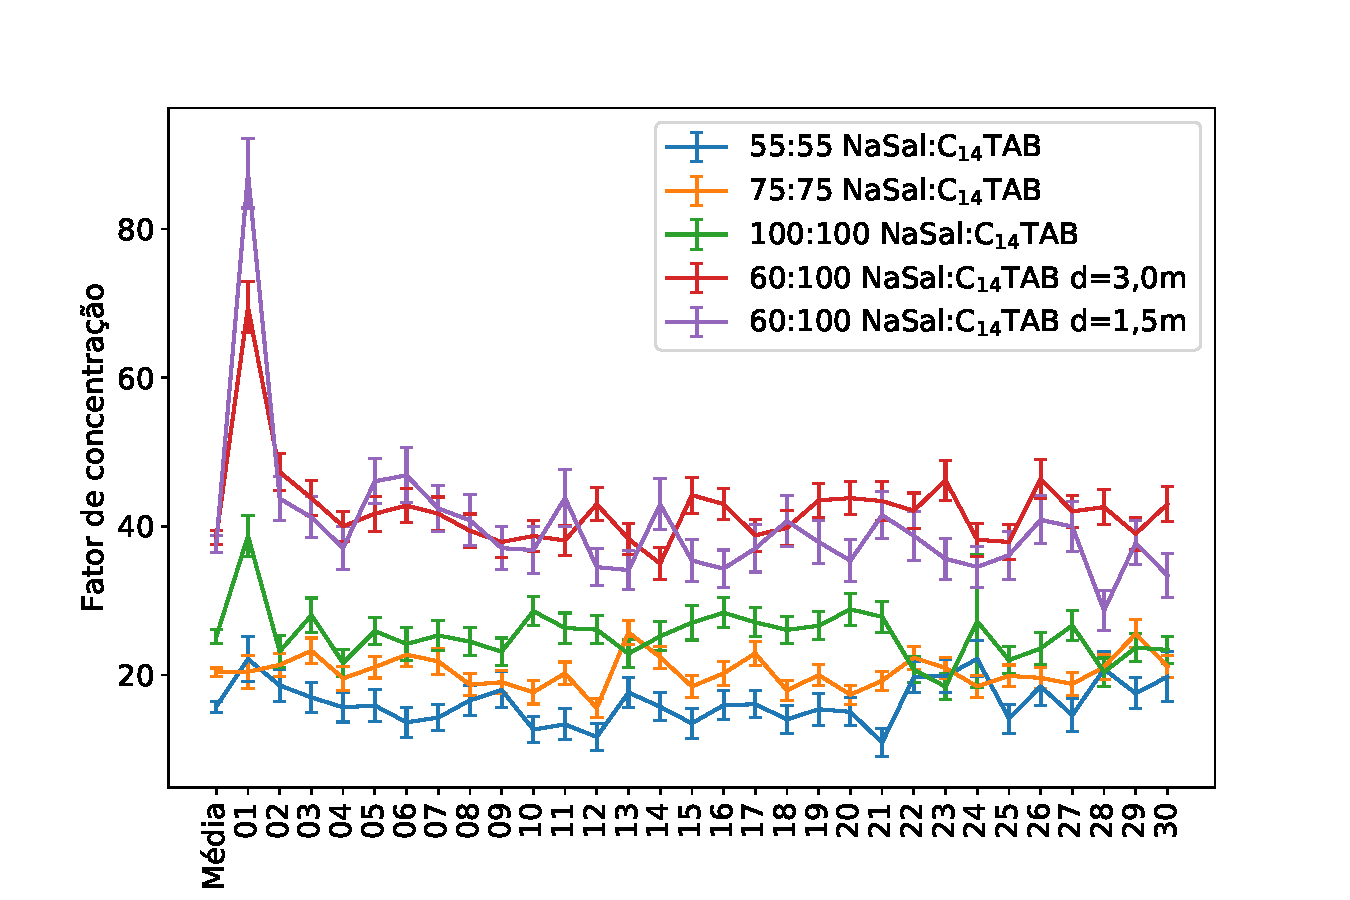
\includegraphics[width=\textwidth]{imagens/saxs/param_nu_rpa}
			\caption{Fator de concentração \(\nu_{RPA}\)}
			\label{fig:param_nurpa}
		\end{subfigure} %
		\begin{subfigure}[t]{0.5\textwidth}
			\centering
			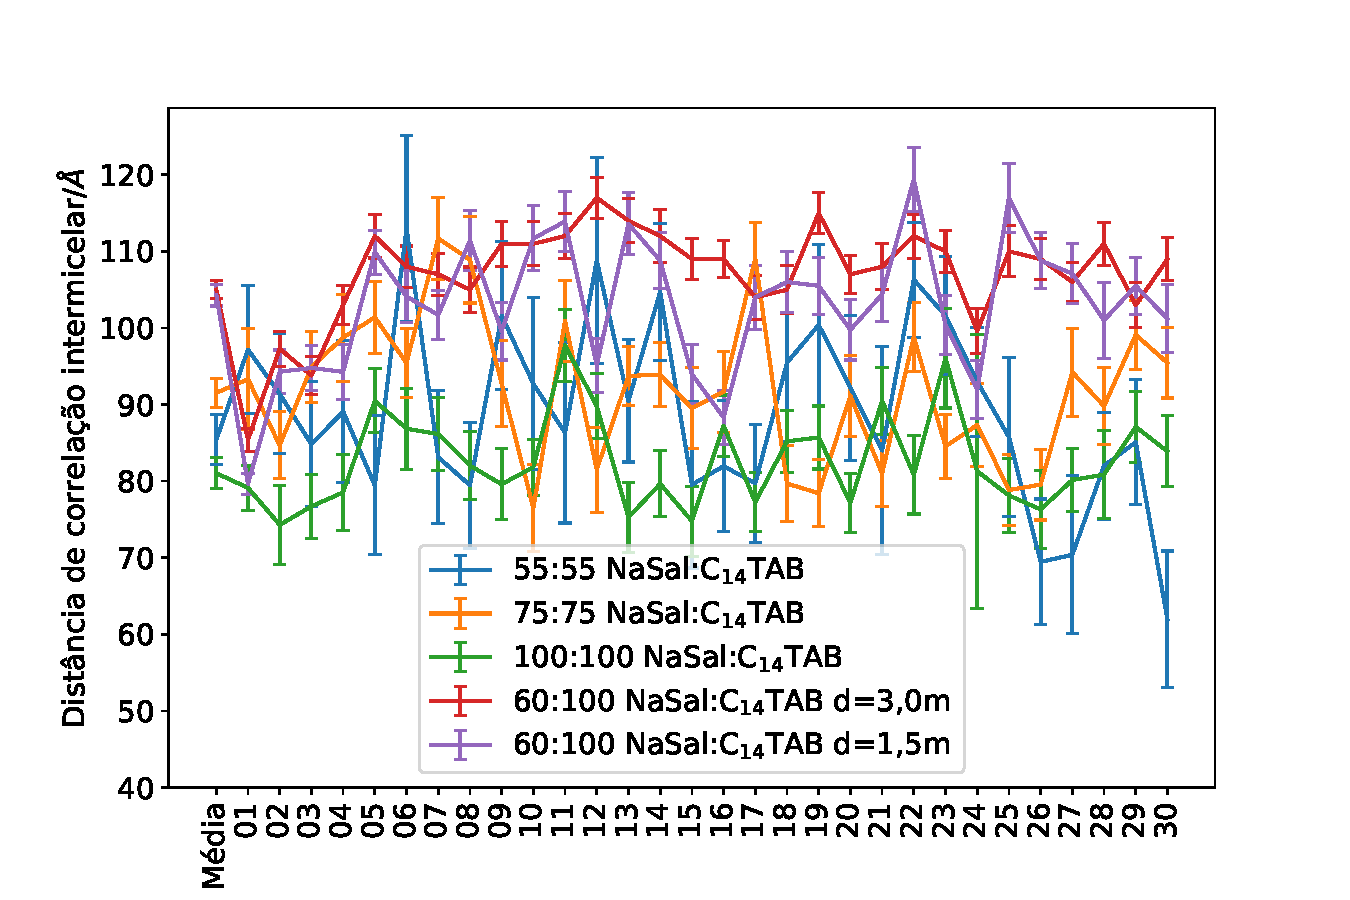
\includegraphics[width=\textwidth]{imagens/saxs/param_d_cq}
			\caption{Distância de correlação \(D_{cq}\)}
			\label{fig:param_dcq}
		\end{subfigure}
		\caption{Parâmetros \(\nu_{RPA}\) e \(D_{cq}\) em nm, das cinco amostras medidas. Os números indicam o \emph{frame}, e o tempo após a mistura pode ser checada na tabela \ref{tab:tr_tempos_frames}. ``Média'' significa o resultado do ajuste da média das curvas 2-30, que eram praticamente idênticas.}
		\label{fig:params_nurpa_dcq}
	\end{figure}

	\begin{figure}
		\begin{subfigure}[t]{0.5\textwidth}
			\centering
			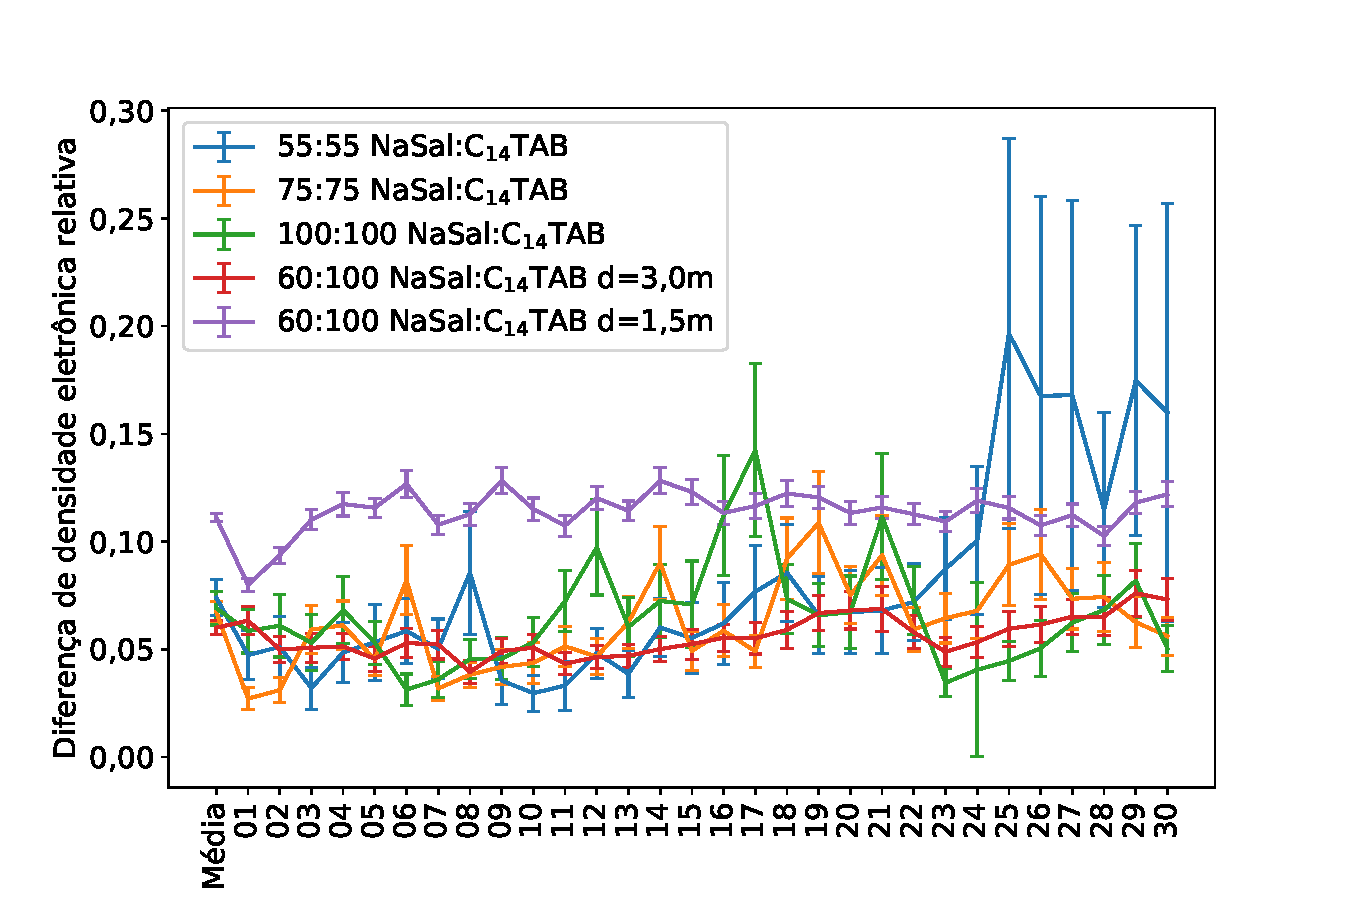
\includegraphics[width=\textwidth]{imagens/saxs/param_rho_rel}
			\caption{Diferença de densidade eletrônica relativa \(\rho_{rel}\)}
			\label{fig:param_rhorel}
		\end{subfigure} %
		\begin{subfigure}[t]{0.5\textwidth}
			\centering
			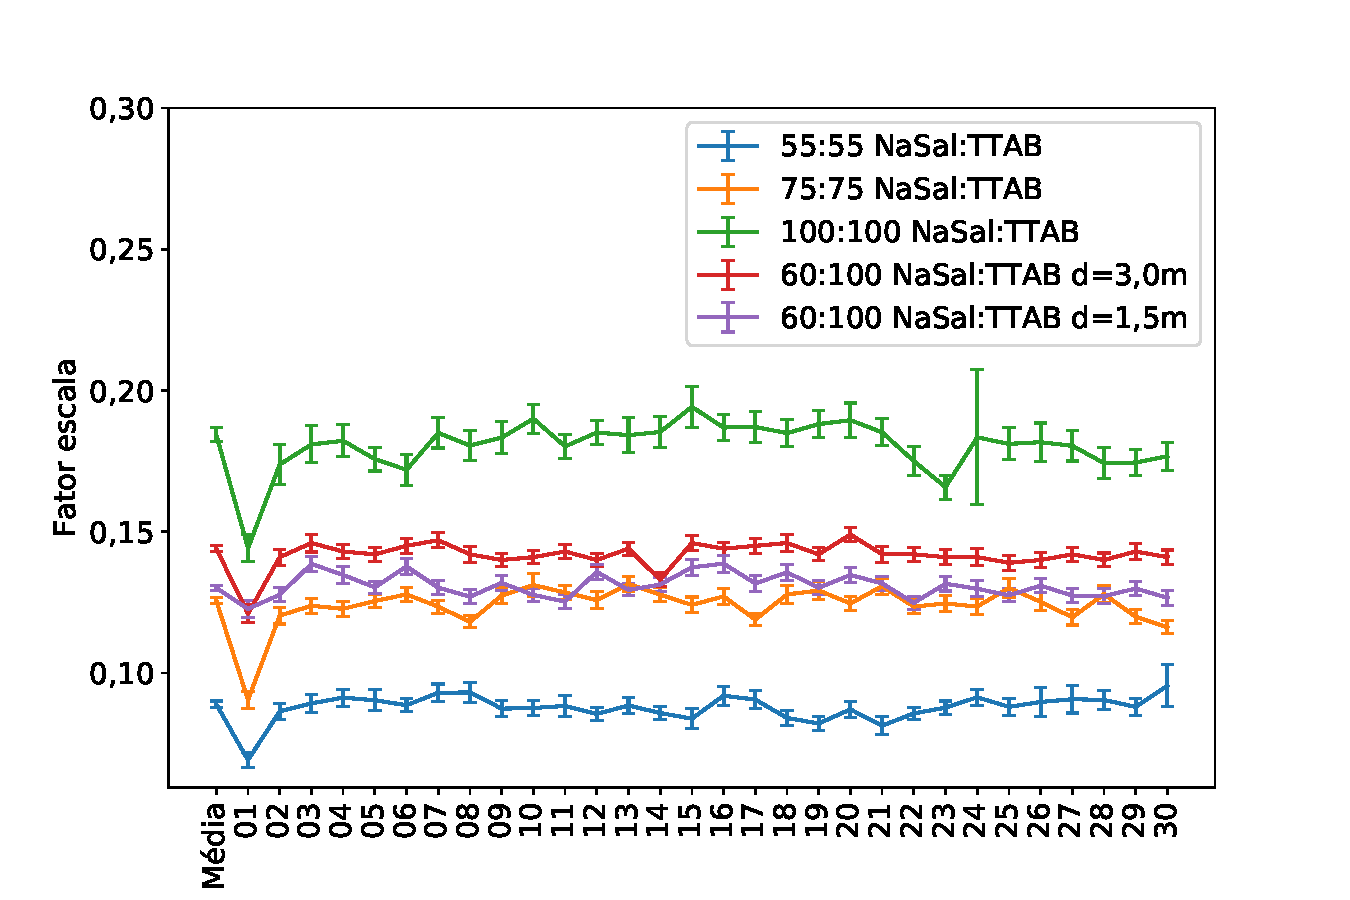
\includegraphics[width=\textwidth]{imagens/saxs/param_scale}
			\caption{Fator de escala}
			\label{fig:param_scale}
		\end{subfigure}
		\caption{Parâmetros \(\rho_{rel}\) e \(scale\) das cinco amostras medidas. Os números indicam o \emph{frame}, e o tempo após a mistura pode ser checada na tabela \ref{tab:tr_tempos_frames}. ``Média'' significa o resultado do ajuste da média das curvas 2-30, que eram praticamente idênticas.}
		\label{fig:params_scale_rhorel}
	\end{figure}

	
	\begin{table}[h]
		\IBGEtab{%
			\caption{Parâmetros de ajuste das curvas de SAXS escolhidos para comparação. Como as curvas 2--30 são praticamente idênticas, foi realizada uma média delas, que depois foi ajustada ao modelo, resultando nos parâmetros aqui.}
			\label{tab:params_ajuste_saxs}
		}%
		{%
			\begin{tabular}{c c | c c c c c c}
				\toprule
				            Composição             & Posição  & Escala/\(10^3\) & \(d_{head}\)/\AA    & \(r_{core}\)/\AA       & \(\rho_{rel}\)   & \(D_{CQ}\)\AA & \(\nu_{RPA}\)      \\ \midrule
				   \multirow{2}{*}{55:55}    & Média    & 89  \(\pm\) 1   & 17,0   \(\pm\) 0,6 & 8,2      \(\pm\) 0,3  & 74   \(\pm\)  8  & 85 \(\pm\) 3  & 15,8   \(\pm\) 0,7 \\
				                             & Primeiro & 69  \(\pm\) 3   & 21   \(\pm\) 1     & 7,4      \(\pm\) 0,7  & 50    \(\pm\) 10 & 97 \(\pm\) 8  & 22,0   \(\pm\) 3,0 \\
				   \multirow{2}{*}{75:75}    & Média    & 126  \(\pm\) 1  & 17,6   \(\pm\) 0,4 & 8,0      \(\pm\) 0,2  & 67   \(\pm\)  5  & 92 \(\pm\) 2  & 20,4   \(\pm\) 0,6 \\
				                             & Primeiro & 90  \(\pm\) 3   & 23,3   \(\pm\) 0,8 & 6,0      \(\pm\) 0,5  & 27   \(\pm\)  5  & 93 \(\pm\) 7  & 20,0   \(\pm\) 2,0 \\
				  \multirow{2}{*}{100:100}   & Média    & 184  \(\pm\) 3  & 17,5   \(\pm\) 0,6 & 8,2      \(\pm\) 0,3  & 69   \(\pm\)  8  & 81 \(\pm\) 2  & 25,2   \(\pm\) 0,9 \\
				                             & Primeiro & 144  \(\pm\) 5  & 19   \(\pm\) 1     & 8,0      \(\pm\) 0,5  & 60    \(\pm\) 10 & 79 \(\pm\) 3  & 39,0   \(\pm\) 3,0 \\
				  \multirow{2}{*}{60:100}    & Média    & 144  \(\pm\) 1  & 19,3   \(\pm\) 0,3 & 8,1      \(\pm\) 0,2  & 60    \(\pm\) 3  & 105 \(\pm\) 1 & 38,5   \(\pm\) 0,9 \\
				                             & Primeiro & 121  \(\pm\) 3  & 20,6   \(\pm\) 0,6 & 8,8      \(\pm\) 0,3  & 63   \(\pm\)  6  & 85 \(\pm\) 1  & 70,0   \(\pm\) 3,0 \\
				\multirow{2}{*}{60:100 1,5m} & Média    & 130  \(\pm\) 1  & 16,4   \(\pm\) 0,1 & 9,99     \(\pm\) 0,05 & 111   \(\pm\)  2 & 104 \(\pm\) 1 & 38,0   \(\pm\) 1   \\
				                             & Primeiro & 123  \(\pm\) 3  & 19,3   \(\pm\) 0,3 & 9,5      \(\pm\) 0,1  & 80    \(\pm\) 3  & 80 \(\pm\) 1  & 87   \(\pm\) 5     \\ \bottomrule
			\end{tabular}
		}{}
	\end{table} 

	Os parâmetros obtidos das amostra 60:100 NaSal:TTAB nas duas distâncias de detector são, em alguns casos, diferentes. Isso ocorre nas medidas da espessura da superfície, raio do \emph{core}, e na diferença de densidade eletrônica. O raio do \emph{core} e da superfície são complementares, e aparecem na região de alto \q, devido ao pequeno tamanho. Logo, as amostras com d=1,5 m, que possuem melhor definição na região de alto \q, também possuem barras de erro menores, em ambos \(r_{core}\) e \(d_{head}\). Além disso, os valores de \(r_{core}\) são maiores para d=1,5 m, mas \(d_{head}\) são complementarmente menores. De qualquer maneira, ambas as distâncias são bastante semelhantes em todas as amostras. Interessantemente, o valor médio da primeira medida é consistentemente diferente das outras, resultado do crescimento das micelas entre o primeiro e os próximos \emph{frames}.
	
	O comprimento da cadeia de surfactante pode ser estimado pela equação de Tanford (Eq. \ref{eqn:tanford}). Com isso, o raio de seção transversal de micelas gigantes com \TTAB{} (\(n=14\)) é de aproximadamente 2 nm, ou 20 \AA. Considerando a presença do grupo trimetilamônio, carregado, e da molécula de salicilato, que pode se posicionar na palisada micelar próximo à superfície ou mais no interior, os tamanhos calculados para \(d_{head}\) e \(r_{core}\) são factíveis, com um raio total de 30 \AA{} (3 nm).
	 % todo: checar se não citei essa equação em lugar nenhum.
	 % todo: ref Israelachvili
	
	\begin{equation}
		l_\mathrm{max} \approx (0,154 + 0,1265n) nm
		\label{eqn:tanford}
	\end{equation}
	
	A diferença entre o primeiro e os últimos \emph{frames} também foi observado no fator de concentração e na distância de correlação. Quanto maior a concentração, maior foi o efeito, e foi máximo no caso onde a composição é 60:100. A diferença entre o primeiro e os últimos frames do fator de concentração pode se dever, ao crescimento das micelas. Antes do crescimento estar finalizado, não há uma rede micelar tão densa, então o fator de concentração é diferente. A distância de correlação, pelo outro lado, mostra que antes do crescimento, a carga superficial micelar era menor, devido à menor distância, e depois se estabilizou. Essas propriedades foram as mais importantes para a diferenciação entre o primeiro \emph{frame} e os demais.
	
	Por último, vemos que a maior parte das amostras possui o parâmetro \(\rho_{rel}\) próximos, com o caso 60:100 1,5 m sendo o mais discrepante. Há uma diferença entre o primeiro e os últimos \emph{frames} possivelmente porque como a incorporação de salicilato não terminou, a diferença de densidade eletrônica da superfície micelar e do interior é diferente. Isso se refletiu no fator de escala, também. Esse parâmetro, porém, não possui muito significado físico, dado que a intensidade do sinal medido não é absoluta.
	
	\FloatBarrier
	
	\section{Conclusão parcial}
	
	Foi possível observar que há uma diferença entre as curvas de saxs obtidas após 35 ms da mistura, e as demais, o que significa que o crescimento micelar foi muito rápido, possivelmente devido à alta concentração do sistema. Essas diferenças foram quantificadas através de ajustes das curvas, das quais foram extraídos parâmetros estruturais das micelas. Infelizmente, observou-se mudanças nos raios da seção transversal das micelas, e não nos comprimentos de Kuhn e de contorno, então não foi possível estimar esses tamanhos.
	
	Para obter resultados de cinética mais adequados, algumas mudanças experimentais podem ser feitas. Na seção \ref{sec:efeito_aditivos_hidrofilicos}, observou-se que a sacarose não afetou a estrutura das micelas. Logo, poderia utilizar-se uma solução de sacarose para aumentar a viscosidade da solução e diminuir a cinética de crescimento. Porém, não se pode aumentar muito a viscosidade, pois há o perigo de estourar o capilar do porta-amostra.
	
	Além disso, a presença de sacarose pode melhorar o contraste, apesar da diferença dos índices de refração entre micela e solvente diminuir. Isso se deve ao fato de que SAXS é dependente da densidade eletrônica total, não somente a densidade eletrônica proporcional ao índice de refração. Além disso, observou-se que TTAB possui um contraste negativo com a água, isso é, espalha menos que o solvente. A presença do 3,4-diclorobenzoato aumentou a densidade eletrônica nas micelas, mas isso resultou numa diminuição do contraste total. % todo: calcular SLD do TTAB e da Água e colocar no texto.
	Sacarose aumentaria a densidade eletrônica do solvente, mantendo a densidade da micela fixa, logo, aumentaria-se o sinal de espalhamento.
	
	Seria possível também utilizar um sistema diferente, que também forma micelas gigantes e que possua, intrinsecamente, maior contraste. Esse foi o caso dos sistemas utilizados na literatura %todo: refs pedersen.
	Isso permitiria que a concentração das espécies seja menor, diminuindo a velocidade da reação. Além disso, caso o sistema tenha contraste o suficiente, seria possível aliar estudos de calorimetria de titulação isotérmica com SAXS resolvido no tempo e o modelo desenvolvido aqui, para correlacionar o crescimento micelar com as várias regiões do entalpograma. Isso permitiria observar, por exemplo, se o crescimento das micelas na região do mínimo do ITC é mais lento do que, por exemplo, numa região com mais surfactante, onde o comprimento micelar final é menor.
	
	
	
	\chapter{Fluorescência resolvida no tempo}